\documentclass{article}
\usepackage{graphicx}
\usepackage{physics}
\usepackage{amsfonts}
\usepackage{amsmath}
%\usepackage{titlesec}
\DeclareMathOperator*{\argmin}{arg\,min}

\title{Investment Management Course Notes}
\author{Joe Hollander}
\date{Summer 2024} 

\begin{document}
\maketitle


\section*{1.1 Fundamentals of risk and returns}

Compounding returns with different return rates:
\[
(1 + r_1)(1 + r_2) - 1.
\]
Compounding returns with the same return rate:
\[
((1 + r)^t - 1). 
\]
To compare different time period standard deviations multiply (or divide)
by the square root of the number of time periods.
The sharpe ratio:
\[
\frac{R_p-R_f}{\sigma_p}.
\]

Pandas standard deviation method uses the sample
standard deviation and not the population standard
deviation. Similar to the sharpe ratio, the calmar
ratior is a risk adjusted return where risk is measured
by drawdown. Use index method to\_period to convert from
datetime to period. Use series method cummax to find the
highest value for each timestep. Drawdown is then: 
\[
\frac{Value - Previous Peak}{Previous Peak}.
\]

\section*{1.2 Beyond The Gaussian Case}

Skew and kurtosis are the third and fourth moments
of a distribution respectively. A distribution with
a greater than three kurtosis is considered fat tailed.

The Jarque Bera is a test that determines whether 
or not a sample distribution fits a normal distribution
based on its skew and kurtosis. If the test is close
to zero it signals that the distribution is close 
to normal. The test:
\[
JB = \frac{n}{6}\left(S^2 + \frac{1}{4}(K-3)^2\right).
\]

Semi-deviation is the volatility of below-average
or below-zero returns:
\[
\sigma_{semi} = 
\sqrt{\frac{1}{N}\sum_{R_t\le\bar{R}}(R_t-\bar{R})^2}.
\]
Value at risk (VaR) represents the maximum
"expected" loss over a time period. A 99\%
one month VaR gives the maximum loss excluding
the 1\% of worst cases. The VaR is also typically
expressed as a positive number. The conditional
value at risk (CVaR) is the expected loss beyond
VaR:
\[
CVar = -E(R \, | \, R \le -VaR).
\]

Setting ddof as zero for pandas standard deviation
calculates the population standard deviation.

There are four methods to calculate VaR.
The historical methodology calculates the VaR 
from the historical outcomes. The parametric gaussian
methodology assumes a gaussian distribution. In
this methodology the VaR is simple to calculate:
\[
VaR_\alpha = -(\mu + z_\alpha \sigma),
\]
where $z_\alpha$ is the $\alpha$-quantile of the
normal distribution with mean zero and standard
deviation one. The gaussian is almost inaccurate.
A parametric non-gaussian distribution doesn't
assume gaussian. The Cornish-Fisher VaR is a
semi-parametric approach. The expansion states:
\[
\tilde{z_\alpha} = z_\alpha + 
\frac{1}{6}(z_\alpha^2 - 1)S + 
\frac{1}{24}(z_\alpha^3 - 3z_\alpha)(K-3) -
\frac{1}{36}(2z_\alpha^3 - 5z_\alpha)S^2,
\] 
where $\tilde{z_\alpha}$ is the updated quantile.

Use numpy's percentile for historical VaR and
scipy.stats' ppf function for gaussian, parametric,
and Cornish-Fisher VaR.

\section*{2.1 Optimization and the Efficient Frontier}

The return of a portfolio is equal to the 
weighted average of the return of the components.
The volatility of a portfolio, however, depends
on the correlation:
\[
\sigma^2(w_a, w_b) =
\sigma^2_A w^2_A + \sigma^2_B w^2_B + 
2 w_A w_B \sigma_A \sigma_B \rho_{A,B}.
\]
The efficient frontier is the boundary of regions
created from the assets with a given correlation.
Each point on this line represents the best return
for each volatility. 

\section*{2.2 Implementing Markowitz}

The capital market line is the tangent line
from the risk free rate to the efficient frontier.
The portfolios from this line have the highest 
sharpe ratio. This maximum sharpe ratio portfolio (MSR)
also has no exposure to unrewarded risks. 

As a result of estimation errors and misleading
expected returns, some use the global minimum variance
(GMV), which is the nose of the efficient frontier. 
Even small estimation errors result in large portfolio
changes. 

\section*{3.1 CPPI and Drawdown constraints}

You cannot diversify out all risk. Dynamic
hedging allows for upside exposure with 
less downside exposure. Correlation often rises when
returns fall. 

The CPPI procedure allows for the construction 
of convex payoffs. The risky asset is a multiplier multiplied by
the cushion. The CPPI is the riskless asset plus the
risky asset. The cushion is then the CPPI minus the protection
floor set in place. Therefore, as the cushion decreases, more
of the portfolio is riskless assets, and as the cushion increases,
more of the portfolio is risky assets. 

\begin{center}
    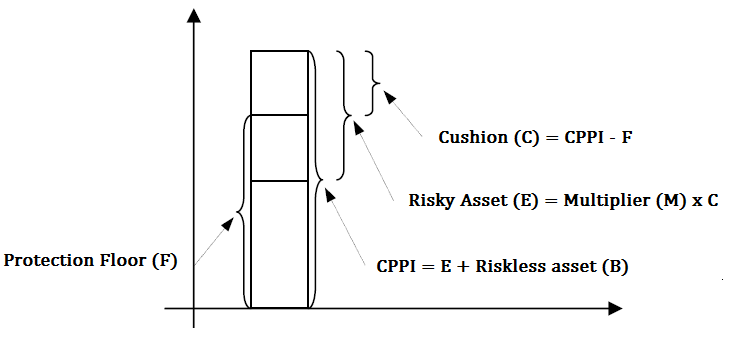
\includegraphics[width=12cm,height=12cm, keepaspectratio]{CPPI.png}
\end{center}

\noindent Gap risk occurs when trading discretely.

Given a max drawdown contraint 
\[V_t > \alpha M_t,\] where: $V_t$ is the value of the portfolio,
$M_t$ is the peak of the portfolio between time $0$ and time $t$,
and $1-\alpha$ is the maximum acceptable drawdown. Then choosing
a multiplier multiplied by $M_t \alpha$ will also provide a convex
payoff. 

A cap can also be used to reduce risk taking passed a value. 
In this system, if the floor is closer, the distance to the floor
is used while if the ceiling cap is closer, the distance to the
ceiling is used. 

Instead of constructing a new DataFrame using an array,
use the DataFrame method reindex\_like.

We can model the return process of a stock $S_t$
with risk-free rate $r$, sharpe ratio $\lambda$,
and volatility $\sigma$: 
\[
\frac{dS_t}{S_t} = 
(r + \sigma \lambda)dt + \sigma dW_t.
\]
For discrete time:
\[
\frac{S_{t+dt} - S_t}{S_t} =
(r + \sigma \lambda)dt +
\sigma \sqrt{dt} \, \xi_t.
\]

\section*{3.2 Monte Carlo}

A more general model of a return process
with the same variables: 
\[
\frac{dS_t}{S_t} = 
\left(r_t + \sqrt{V_t} \, \lambda_t^S\right)dt +
\sqrt{V_t} \, dW_t^S.
\]

We can also define the risk-free rate and variance
in terms of brownian motion: 
\begin{gather}
    dr_t = a(b-r_t)dt + \sigma_r dW_t^r \nonumber \\
    dV_t = \alpha(\bar{V} - V_t)dt + 
    \sigma_V \sqrt{V_t} \, dW_t^V \nonumber
\end{gather}
Here, $b$ is the long term mean of the risk-free rate.
Both of these processes are mean reverting. 

In a CPPI system, raising the risky-asset multiplier
when the market is less volatile and vice-versa results
in less breaches of the floor and less need for 
rebalancing more frequently. 

\section*{4.1 Asset-Liability Management}

The funding ratio $F_t = {A_t}/{L_t}$ and surplus
$S_t = A_t - L_t$ is what really matters
for asset-liability management.  

The present value of a set of liabilities is
\[
PV(L) = \sum_{i=1}^k B(t_i)L_i,
\]
and if the yield curve is flat, 
the price of a pure discount bond is 
\[
B(t) = \frac{1}{(1+r)^t}, 
\]
where $r$ is the annual rate of interest. 

Liability-hedging portfolios attempt to match the cashflows of
the liability side in order to pay liabilities in the future. 
Often, cash-flow matching is not feasible or practicle, so one may
use factor exposure matching. These factor exposure matching portfolios
often use bonds to gain similar exposure to interest rates that affect
liabilities. 

The Cox Ingersoll Ross (CIR) model that is used to model interest rates:
\[
dr_t = a(b-r_t)dt + \sigma \sqrt{r_t} \, dW_t,
\]
where $b$ is the long term mean of the interest rate. 

Since performance generation and hedging are incompatible aims,
creating a performance-seeking portfolio (PSP) and
a liability-hedging portfolio (LHP) is the best option.
This two portfolio style is called liability-driven investing (LDI).
The formal expression of the goal is:
\[
\max_w E \left[u\left(\frac{A_t}{L_t}\right)\right]
=> w^* = \frac{\lambda_{PSP}}{\gamma \sigma_{PSP}}w^{PSP}
+ \beta_{L,LHP} \left(1-\frac{1}{\gamma}\right)
w^{LHP}.
\]
The greeks of LDI are these greek letters. $\lambda_{PSP}$ 
is the sharpe ratio of the PSP, $\gamma$ is the risk aversion,
$\sigma_{PSP}$ is the standard deviation of the PSP,
$\beta_{L,LHP}$ is the beta of the liabilities with respect to the LHP.

\section*{1.2 Introduction to Machine Learning}

Aqequate data is needed for a train-test split, and
data must be stable (stationary). 
While traditional statistics builds model and relies
on assumptions, machine learning relies on large data. 

Taking the average classification of multiple classifiers
does best with respect to reducing estimation errors.
Implementing a voting system, called boosting, is another way
to combine different classifiers. 

Dimensional reduction such as PCA helps with feature selection.
Clustering algorithms can also be used. 

\section*{2.1 Introduction to Factor Models}

Macro-factors such as GDP growth, interest rate, and inflation
are applicaple to many asset classes. Micro-factors, on the 
other hand, are only applicable to specific asset classes. 
Investing with an aim for diverse factor exposure is better than
investing for general diversification as different asset classes
may have the same factors. 

The simplest factor model, the market model:
\[
R_{i,t} - r_{f,t} = \alpha_i + \beta_i(R_{M,t} - r_{f,t}) + \epsilon_{i,t},
\]
where  $r$ is the risk-free rate, $R_{i, t}$ is the return of the specific asset,
and $R_{M,t}$ is the return of the market. The explanatory 
power or $R^2$, is the part of the variance explained by the 
factor model: 
\[
R^2 = \frac{\beta_i^2 \sigma_M^2}{\sigma_i^2}.
\]

A multi-factor model then relates the excess return of the 
asset to the excess return of other factors:
\[
R_{i,t}-r_{f,t} = \alpha_i + \beta_{i,1}F_{1,t} + ... + \beta_{i,k}F_{k,t} + \epsilon_{i,t}.
\] 
Fama and French's 1992 model used this to show that stocks'
market cap, market size, and value were statistically significant 
in predicting returns. The momentum factor is also a highly
recognized factor. 

Instead of calculating covariance for a large number of assets,
we can estimate covariance as a function of exposure to the factors:
\begin{gather}
    \sigma_{ij} = cov(R_i, R_j) = \sum_{k=1}^K \beta_{ik} \beta_{jk} \sigma_k \nonumber \\  
    \sigma_{ii} = cov(R_i, R_i) = \sum_{k=1}^K \beta_{ik}^2 \sigma_{F_k}^2 \nonumber.
\end{gather}
This assumes uncorrelated factors and uncorrelated residuals, but 
it also leads to less estimation errors and overfitting.

\section*{2.2 Estimation of Factor Models}

A penalty method called ridge regression is used to prevent 
overfitting from overly high coefficients. In the equation:
\[
\hat{\beta}(\lambda) = \argmin_\beta \{|| y - X\beta ||^2 + \lambda ||\beta||^2\},
\]
$\lambda$ is the penalty term and as the $||\beta||$, the normed sum of coefficients,
increases the model is penalized. The lasso method is similar, 
except the normed $\beta$ isn't squared. Finding a middleground
penalty term $\lambda$ is important.

Train and test, a cross-validation method, involves testing on
a different subset of the data and taking the average of the performance.
Each subset is often called a fold. 

Penalty terms are one type of shrinkage. Stein's paradox states
that when estimating three or more paramaters, the best model
is the average of three parameters as this lowers variance
and minimizes the mean squared error. This shows that biasing
and shrinking are useful in minimizing error.

In scikit-learn, instead of $\lambda$ they use
\[
\alpha = \frac{\lambda}{2n}. 
\]
Additionally, the formulas for their ridge and lasso regressions
are different. 

Best subset regression is a regression method that constrains
the number of factors.

\section*{3.1 Measuring Diversification}

Unsupervised learning can be used to more accurately measure
diversification. This is especially useful as diversification
can change over time.

The effective number of constinuents can be measured as such:
\[
ENC \equiv \frac{1}{\sum_{i=1}^{N}w_i^2}.
\]
This shows that because the S\&P 500 is market cap weighted,
it only has about 100 effective constituents. Instead of 
measuring a portfolio as a portfolio of assets, we can measure
it as a portfolio of factor exposure. The effective number of
bets is then given by:
\[
ENB = \frac{1}{\sum_{i=1}^{N}p_k^2},
\]
where \[p_k = \frac{w_{F_k}^2\sigma_{F_k}^2}{\sigma_p^2}.\]
In the former equation, $\sigma_p^2$ is the variance of the
portfolio.

\section*{3.2 Maximizing Diversification Benefits}

Sparce PCA is a machine learning alternative 
to traditional PCA. Clustering, another unsupervised
learning method, seeks to minimize the distance between points
and their clusters' median. 

Conditional independence is a concept where two objects
may be related by a mutual connection but are independent of
each other. The conditional independence of two variables $x$
and $y$, given that $z$ has occured:
\[
X \perp Y \,|\, Z \Leftrightarrow P(x,y\,|\,z) = P(x\,|\,z)P(y\,|\,z).
\]
The precision matrix is the inverse of the correlation
matrix, and if the entry is zero, then the two variables 
are conditionally independent.

Improving sparsity helps with diversification and can be
achieved by using lasso a penalty function. Testing this
concept on the top 50 stocks in the S\&P 500,
we find that clustering and PCA yield the highest
sharpe ratio and returns.   

There is no need to know the number of clusters for the affinity
propogation algorithm while the number of clusters must be known
for k-means. Multi dimensional scaling allows for visulization 
of multi dimensional data in to two dimensions. 

\section*{4.1 Varying Market Conditions}

Since correlations increase in crash periods,
identifying these regimes can be helpful with
risk management and portfolio choice.

A GARCH model tries to model the current variance
based on the long-run variance rate $V_L$:
\[
\sigma_T^2 = \gamma V_L + 
\sum_{t=1}^T \alpha_t R_t^2 + \beta \sigma_{T-1}^2,
\]
where
\[ \gamma + \beta + \sum_{t=1}^T \alpha_t = 1,\]
and \[ \alpha_t = \frac{\lambda^{T-t}}{\sum_{t=1}^T \lambda^{T-t}.}\]
The lower the lambda the higher the weight assigned to recent
observations. 

A markov regime switching model implies that volatility is
not a function of time but a function of a state. 
The parameters of the transition matrix can be estimated 
my maximizing log likelihood. Machine learning can also be used
for non-parametric identification.

\section*{4.2 Regime Switching with Machine Learning}

Even two regime models perform much better at forecasting
the tails of returns. A long term model is one that uses
a historical transition matrix. The optimization problem to solve
is this:
\[
\hat{\beta} = \argmin_\beta  || x-\beta||_2^2 + \lambda||D\beta||_1. 
\]
In this equation, $\hat{\beta}$ is the updated values of the timeseries.
If we increase $\lambda$ the timeseries must be flat, and if we 
decrease $\lambda$ to zero than the series must be equal to $x$. 

\section*{5.1 Traditional Statistics and Machine Learning}

Traditional regression models are often ineffective
at forecasting crash periods. 


Logisitc regression is often used for binary classification as 
it gives a probabliity measure: 
\[
h_\beta = \frac{1}{1+e^{-(\beta_0 + \beta x)}}.
\]
Typically, the final classification is done by choosing 
a threshold value. To learn this model we maximize
the maximum-likelihood where $y_i$ is the predicted class/state:
\[
J(\beta) = \sum_{i=1}^N y_i\log(h_\beta(x_i)) + (1-y_i)\log(1-h_\beta(x_i)).
\]

To create sparsity, decrease variance, improve a model, 
and prevent overfitting, there are many ways. 
Elastic net, a model with two penalty terms, is best when features
are correlated. Stepwise regression, a model that increases the degree of each
polynomial term, is another alternative. Subset selection,
a method where the model is built with only a certain amount of 
paramaters, is another method to reduce overfitting. Using an ensemble method
to combine multiple models is also useful. 

For k-nearest neighbors (k-NN), the k defines how many neighbors
will be used to classify the point. Training errors often increase
with k. The algorithm can use euclidean distance (L-2 norm)
or manhattan distance (L-1 norm). 

A decision tree divides the data into subsets on feature at a time.
It does this by selecting the feature level that best splits
the data. The algorithm can be used for regression or classification.

Boosting is a machine learning algorithm that combines multiple
models. It does this by creating a weak learning model and then
creating more models that have loss functions that reward
getting high error datapoints more correct. It then iteratively 
creates more models and finds a weighted average of the prediction.
The higher the error of the model, the lower the weight in the voting
system. 

\section*{5.2 Predicting Crash Regimes}

Several different models were used to attempt to predict
if the next month would be a crash regime or not. Logistic regression
did poorly, k-NN performed amazing, decision tree did worse than k-NN, and
gradient boosting did slightly worse than k-NN. An ensemble model
performed better than most of the models but still worse than k-NN.

Balanced and imbalanced data refers to the distribution of classes
in the data. In a typical two state, growth and constraction model, 
the data is imbalanced. 

The ROC metric represents the true positive rate (TPR) and
the false positive rate (FPR):        
\begin{center}
    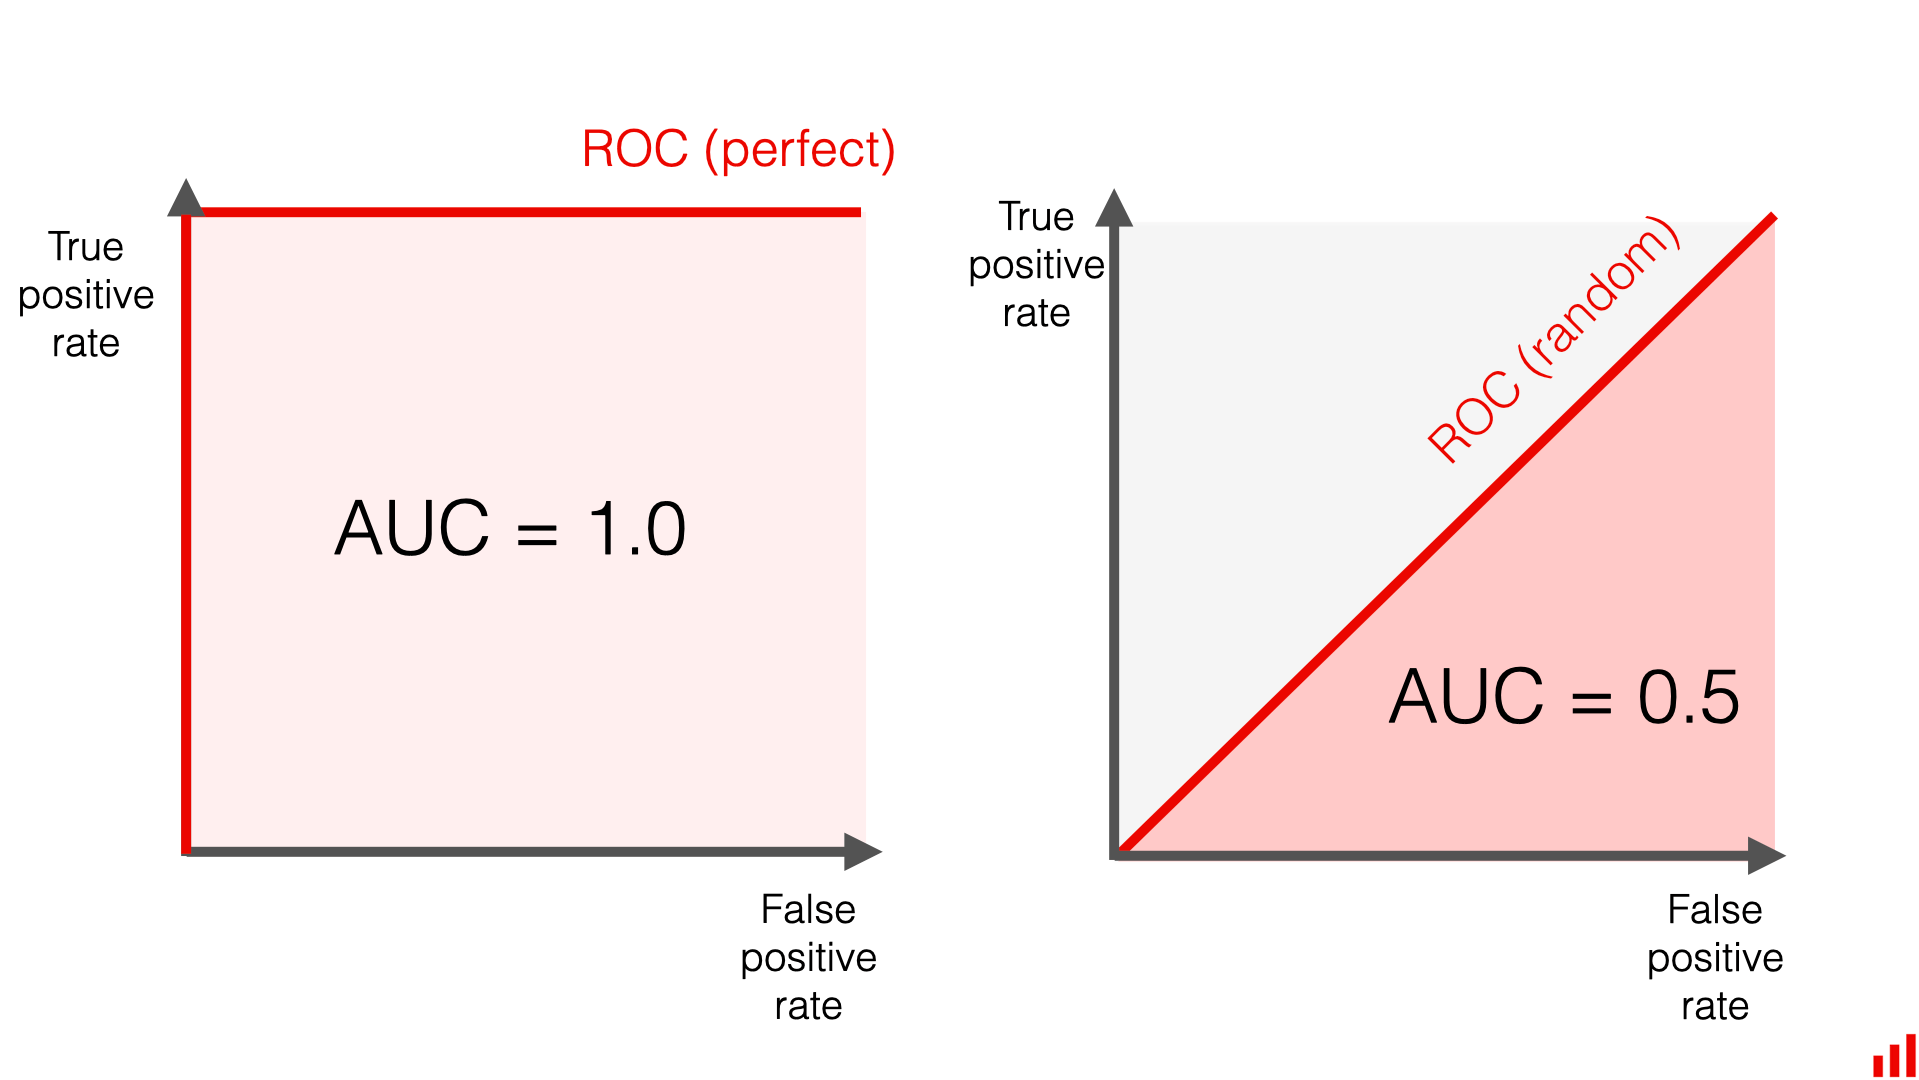
\includegraphics[width=12cm,height=12cm, keepaspectratio]{ROCmetric.png}
\end{center}

\begin{center}
    
\end{center}

\end{document}